% !TEX root = ../pdf/stat205.tex
% [There are multiple stat205.tex files, but the one in ../pdf is the usual one]



%%%%%%%%%%%%%%%%%%%%%%%%%%%%%%%%%%%%%%%%%%%%%%%
\chapter{Probability Distributions}


\begin{verse}{\it
``When there are but two players, your theory which proceeds by combinations is very just. \\
But when there are three, I believe I have a proof that it is unjust that you should proceed in any other manner than the one I have.''\vspace*{6pt}} \\
\hspace*{2cm} -- Pascal's letter to Fermat\FOOTNOTE{from \url{https://www.york.ac.uk/depts/maths/histstat/pascal.pdf}}
\end{verse}
\vspace*{12pt}


\section{Random Variables}

In Example \autoref{exmp:three_fair_coins}, we denote the number of observed heads by \( \bm{X} \),
which can take on values 0, 1, 2, or 3.
Each of these numbers corresponds to one of the following events:
\begin{itemize}
    \item 0: \( A = \{ TTT \} \),
    \item 1: \( B = \{ HTT, THT, TTH \} \),
    \item 2: \( C = \{ HHT, HTH, THH \} \),
    \item 3: \( D = \{ HHH \} \)
\end{itemize}
In other words, the sample space is partitioned into events \( A, B, C, \) and \( D \).
Hence, we can map each element of \( S \) to exactly one element of \( \{ 0, 1, 2, 3 \} \).
This mapping is achieved using \( \bm{X} \), which is called a \keyterm{random variable}.

Thus:
\begin{gather*}
    X(TTT) = 0, X(HTT) = X(THT) = X(TTH) = 1, X(HHT) = X(HTH) = X(THH) = 2, X(HHH)= 3
\end{gather*}

More formally, in a probability model with sample space \( S \),
a random variable (or simply a variable) is a real-valued function \( X: S \rightarrow R \),
where the range of \( \bm{X} \) is a subset of the real numbers.
The range of \( \bm{X} \) is called the \keyterm{support} of \( \bm{X} \) and is denoted by \( S_{\bm{X}} \).

Conventionally, if \( A \subset R\), we define:
\begin{gather*}
    (\bm{X} \in A) = \{ e \in S | \bm{X}(e) \in A \}
\end{gather*}
For instance, in the previous example, \( (\bm{X} < 2) = (\bm{X} \in (-\infty, 2)) = (\bm{X} \in \{ 0, 1 \}) = \{ TTT, HTT, THT, TTH \} \).

When working with random variables, probabilities can be described quantitatively.
For example, if we want the probability that the number of heads is fewer than 2, we are interested in the event \( (\bm{X} < 2) \).
As shown earlier, this corresponds to:
\begin{gather*}
    P(\bm{X} < 2) = P(\bm{X} \in \{ TTT, HTT, THT, TTH \}) = \frac{4}{8} = \frac{1}{4}
\end{gather*}

\begin{exmp}
    Suppose in Example \autoref{exmp:heads_observe}, \( \bm{X} \) is the number of coin tosses required to observe the first heads.
    Thus, the support of \( \bm{X} \) is \( S_{\bm{X}} = \{ 1, 2, \ldots \} \).
    For instance, if one iteration of this experiment yields the outcome \( TTTH \),
    then \( \bm{X}(TTTH) = 4 \), as the first heads occurs on the fourth toss.

    The probability that the number of coin tosses required to observe the first heads is an odd number is given by:
    \begin{align*}
        P(\bm{X} \in \{ 1, 3, \ldots \}) &= P(\{ H, TTH, \ldots \})\\
        &= P(\{ H \}) + P(\{ TTH \}) + \ldots\\
        &= (\frac{1}{2}) + (\frac{1}{2})^3 + \ldots\\
        &= \frac{2}{3}
    \end{align*}
\end{exmp}

\begin{exmp}
    In the previous example, what is the probability that more than six coin tosses are required to observe the first heads?
\end{exmp}

In the two examples we analyzed so far, the support \( S_{\bm{X}} \) is countable.
In this case, we say \( \bm{X} \) is a \keyterm{discrete random variable}.
Conversely, if a random variable can take on infinitely many (uncountable) number of values,
we call it a \keyterm{continuous random variable}.

Below are examples of continuous random variables:

\begin{exmp}
    In Example \autoref{exmp:lightbulb_lifespan}, let \( \bm{X} \) be lightbulb's lifespan.
    Since lifespans can take any non-negative real value, \( \bm{X} \) is a continuous random variable.
\end{exmp}

\begin{exmp}
    Suppose a needle is dropped at random into a circular disk of radius 3.
    The sample space consists of all possible landing positions of the needle, which are uncountable.
    Let \( \bm{X} \) denote the distance from the needle's landing point to the center of the disk.
    Then \( \bm{X} \) is a continuous random variable with support \( S_{\bm{X}} = [0, 3] \),
    where the interval includes the boundary points (accounting for the possibility of landing exactly on the disk's edge).
\end{exmp}

\section{Probability Distribution}

We saw that different values of a random variable \( \bm{X} \) implicitly partition the sample space into mutually exclusive events.
A key characteristic of any probability model is the probability it assigns to each possible value of the random variable.
When \( \bm{X} \) is discrete (taking on countably many values), we can conveniently represent its \keyterm{probability distribution} using a graph, a table, or a function.
\begin{exmp}\label{exmp:three_dice_prob_dist}
    The probability distribution table for \( \bm{X} \) (the number of observed heads) in Example \autoref{exmp:three_fair_coins} is:
	\begin{center}
	\begin{tabular}{|c|c|c|c|c|c|}
	\hline
	\( \bm{x} \) & 0 & 1 & 2 & 3 & Total \\
	\hline
	\( P(\bm{X} = \bm{x}) \) & \( \frac{1}{8} \) & \( \frac{3}{8} \) & \( \frac{3}{8} \) & \( \frac{1}{8} \) & \( 1 \) \\
	\hline
	\end{tabular}
	\end{center}
    Note that the sum of all assigned probabilities equals 1, as expected.

    The corresponding graph is shown in \autoref{fig:three_dice_prob_dist}.
    \begin{figure}[t]
    \begin{center}
    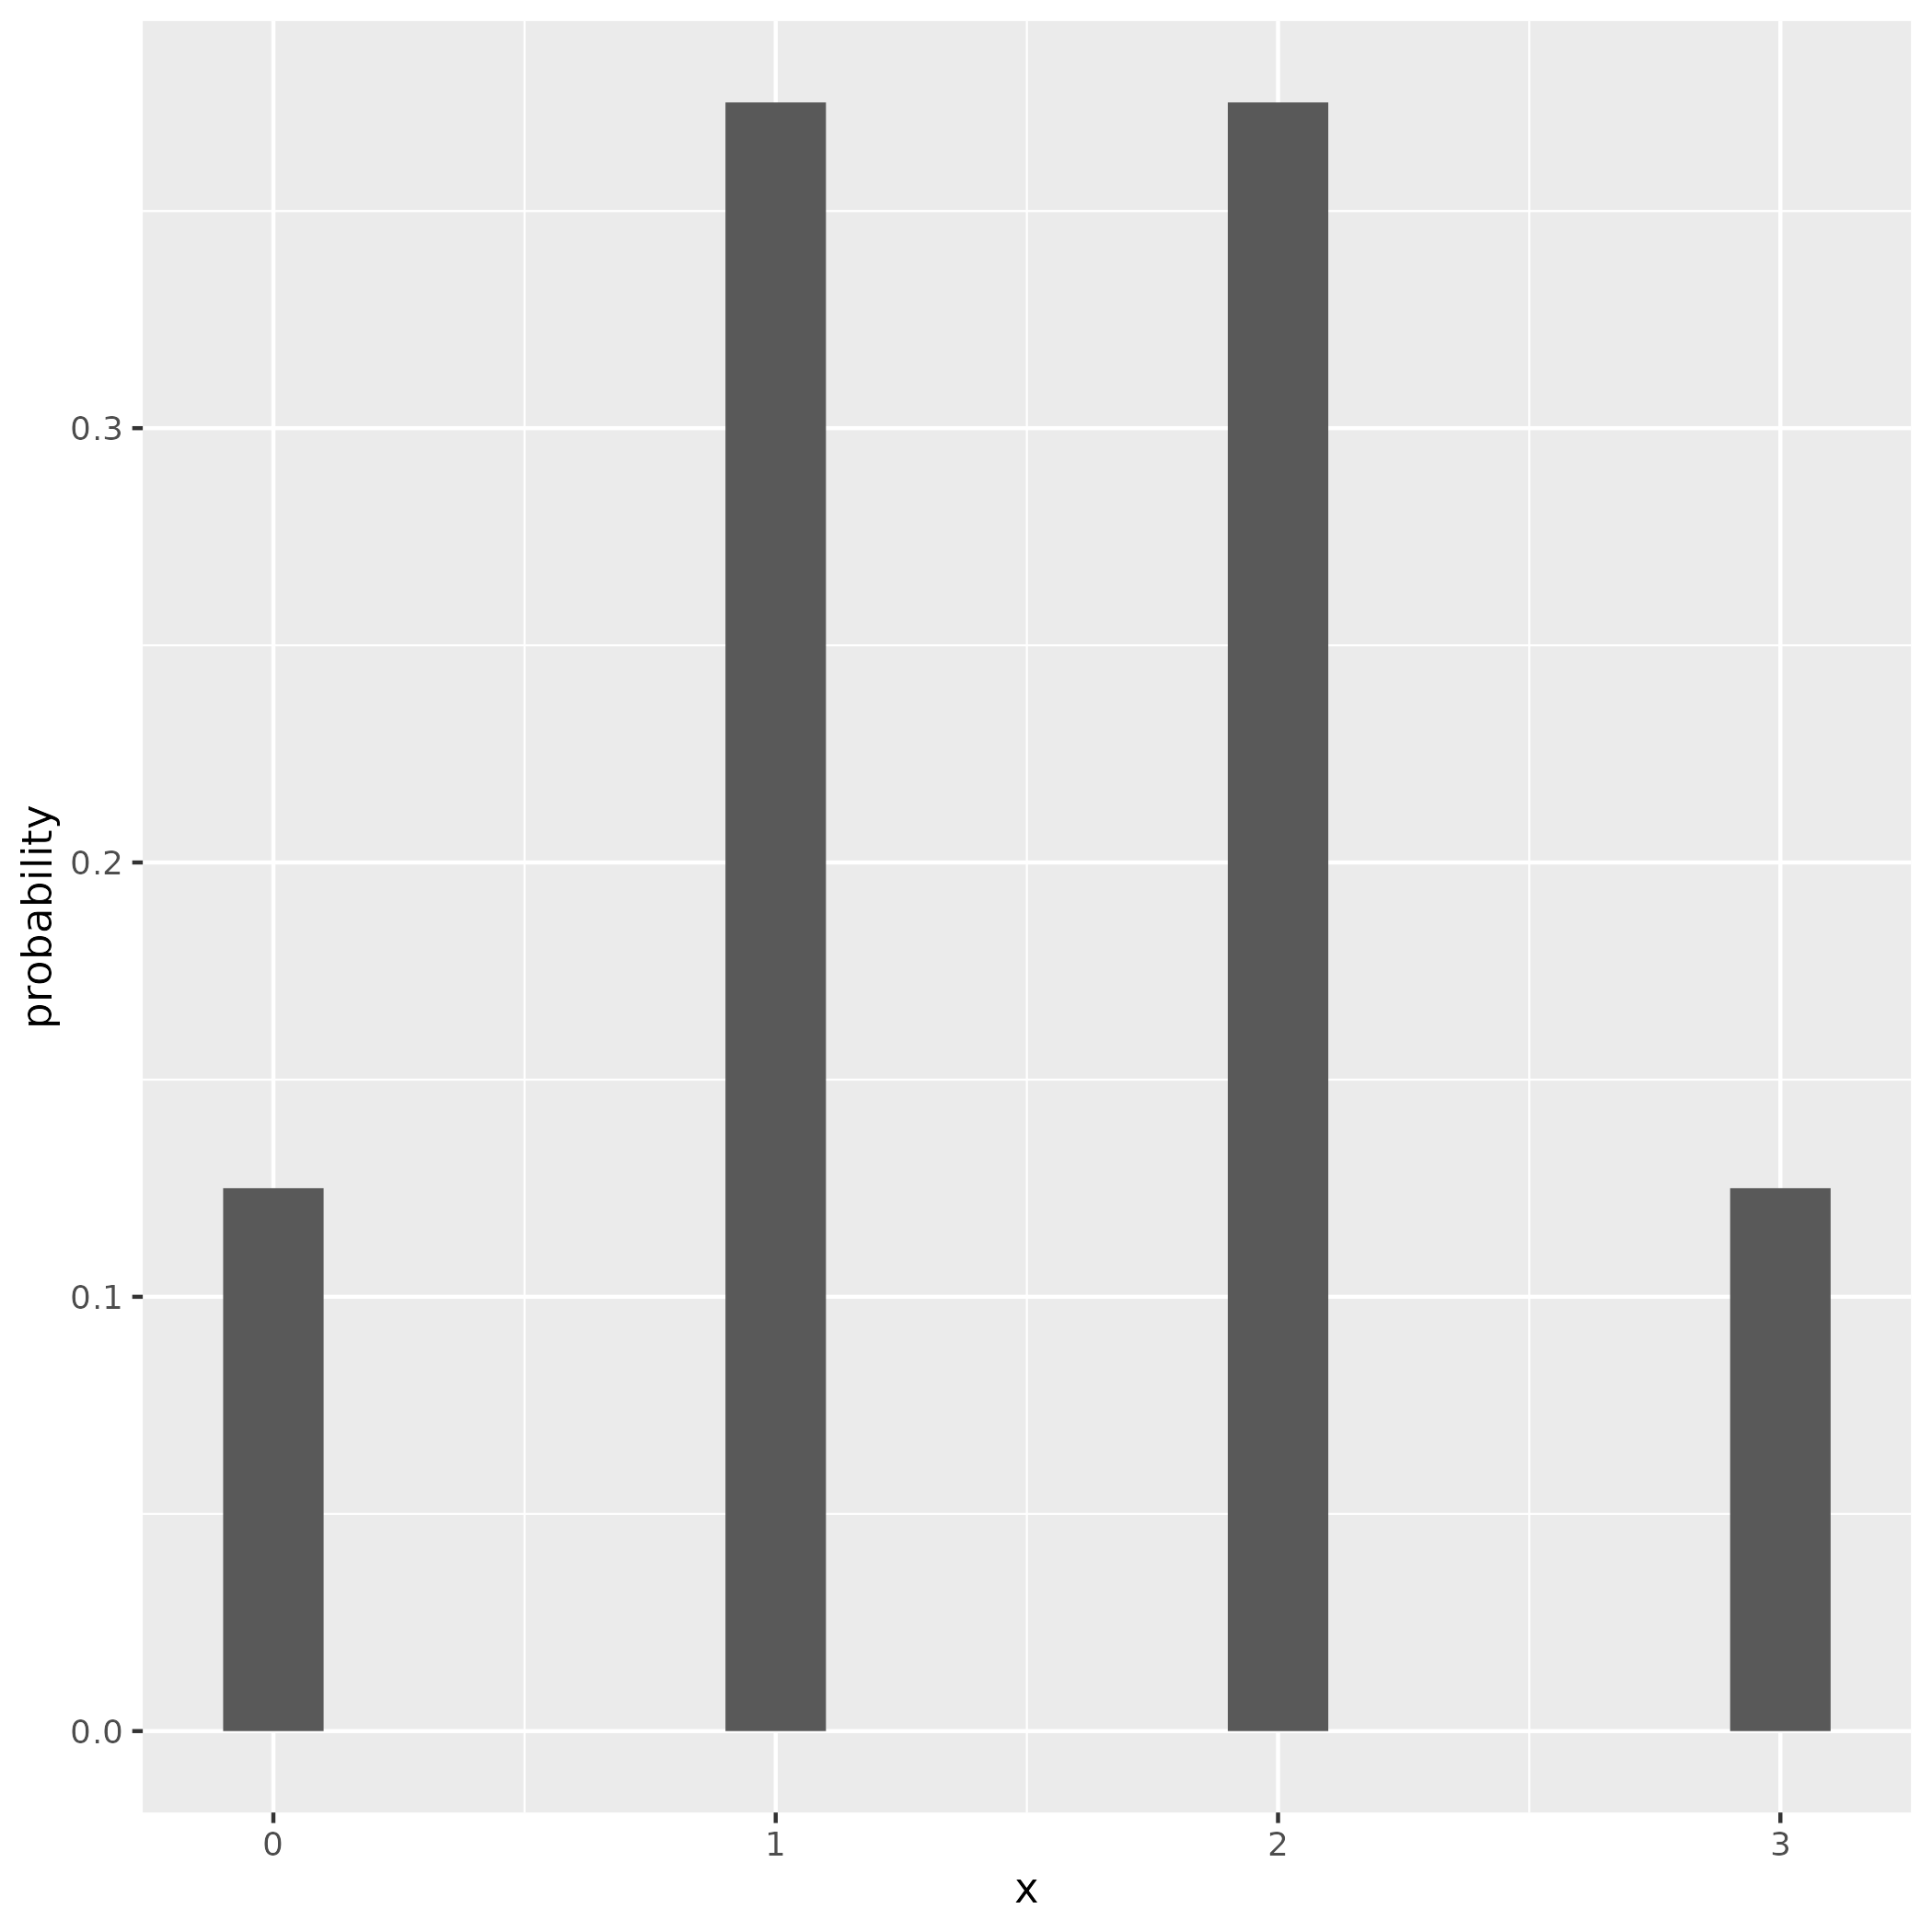
\epsfig{file=../img/threeDiceProbDistrib.png,clip=true,width=8.8cm}
    \end{center}
    \caption{Probability distribution graph for Example \autoref{exmp:three_dice_prob_dist}}
    \label{fig:three_dice_prob_dist}
    %\HR
    \end{figure}
\end{exmp}
For a discrete random variable \( \bm{X} \), we can also describe its probability distribution using a function.
This function is called \keyterm{probability mass function (PMF)}, and is defined as follows:
\begin{align*}
    p_{\bm{X}} \colon R &\to [0, 1] \\
    \bm{x} &\mapsto P(\bm{X} = \bm{x})
\end{align*}
where \( P \) is a probability measure.

All values of \( \bm{X} \) without assigned probabilities are implicitly defined to be zero.
For instance, in the previous example, the PMF is:
\begin{gather*}
    p_{\bm{X}}(\bm{x}) = \begin{cases}
        \frac{1}{8}, & \text{if } \bm{x} = 0, 3\\
        \frac{3}{8}, & \text{if } \bm{x} = 1, 2\\
        0, & \text{O.W.}\\
    \end{cases}
\end{gather*}
Henceforth, when specifying a probability mass function (PMF), we will omit all values of the random variable that have zero probability.

\section{Discrete Distributions}

Many problems we encounter follow the same pattern in how they assign probabilities to different values of a random variable.
Here, we discuss two such cases for discrete random variables.

\subsection{Bernoulli Distribution}

In a coin toss, the outcome is either heads or tails (Example \autoref{exmp:coin_toss}).
When drawing a ball from an urn containing only blue and red balls, it's either red or blue.
When selecting a lamp from the box for quality inspection, each lamp is either functional or defective.

These are all examples of \keyterm{Bernoulli trial}, where an experiment yields exactly one of two possible outcomes.
We designate one outcome as a "success" (typically mapped to 1) and the other as a "failure" (mapped to 0).
The corresponding Bernoulli random variable \( X \) thus has the probability mass function:
\begin{gather*}
    p_{\bm{X}}(\bm{x}) = \begin{cases}
        p, & \text{if } \bm{x} = 1\\
        1 - p, & \text{if } \bm{x} = 0\\
    \end{cases}
    = p^x(1 - p)^{1 - x}
\end{gather*}
where \( \bm{x} = 0, 1 \) and \( p \) is the probability of success.
We call \( \bm{X} \) a \keyterm{Bernoulli random variable}, and we write \( \bm{X} \sim Bern(p) \), indicating that X follows a \keyterm{Bernoulli distribution} with success probability \( p \).
\begin{exmp}
    Consider an unfair coin toss where the probability of landing heads is \( \frac{2}{3} \).
    Let \( \bm{X} \) be the random variable representing the observation of heads. Then \( \bm{X} \sim Bern(\frac{2}{3}) \).
\end{exmp}
\begin{exmp}
    For a fair six-sided die roll, let \( X \) be the indicator random variable for the event "not six."
    The success probability is observing 1, 2, 3, 4, or 5,
    which is \( p = \frac{5}{6} \),
    and thus \( \bm{X} \sim Bern(\frac{5}{6}) \).
\end{exmp}

\subsection{Binomial Distribution}

Suppose \( n \) identical Bernoulli trials are preformed independently from each other.
If \( \bm{X} \) is the number of successes in these \( n \) trials, then it is called a \keyterm{binomial random variable}.
We say \( \bm{X} \) follows a \keyterm{binomial distribution} and denote this by \( \bm{X} \sim B(n, p) \),
where \( p \) is the probability of success and remains the same in each Bernoulli trial.

To compute the \( \bm{X} \)'s PMF \( p_{\bm{X}}(\bm{x}) \),
we first choose \( \bm{x} \) trials out of total \( n \) Bernoulli trials.
This can be done in \( n \choose x \) ways.
Now consier any one of these arrangements of \( \bm{x} \) successes and \( n - \bm{x} \) failures.
The following analysis focuses on the configuration depicted in \autoref{fig:binom_seq}.
\begin{figure}[t]
\begin{center}
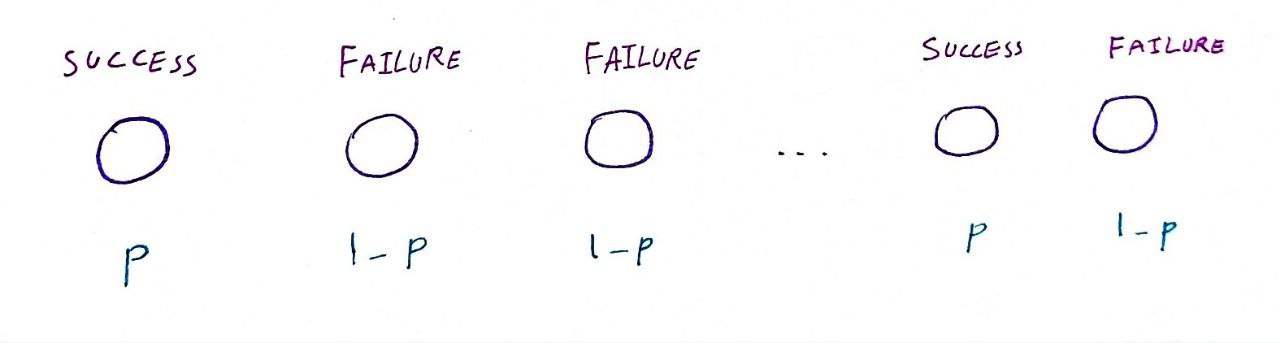
\epsfig{file=../img/binomSeq.jpg,clip=true,width=8.8cm}
\end{center}
\caption{one arrangement of \( \bm{x} \) successes and \( n - \bm{x} \) failures in \( n \) independent Bernoulli trials}
\label{fig:binom_seq}
%\HR
\end{figure}
What is the probability of such a sequence occurring?

Let \( S_i \) denote the event of success in the \( i \)-th trial and \( F_i \) the event of failure, where \( i = 1, 2, \ldots, n \).
Since the trials are independent from each other, the multiplcation rule yields:
\begin{align*}
    P(S_1 \cap F_2 \cap F_3 \cap \ldots \cap S_{n - 1} \cap F_{n}) &= P(S_1)P(F_2)P(F_3)\ldots P(S_{n - 1})P(F_n)\\
    &= p(1 - p)(1 - p)\ldots p(1 - p)\\
    &= p^{\bm{x}}(1 - p)^{n - \bm{x}}
\end{align*}
Thus:
\begin{gather*}
    p_{\bm{X}}(\bm{x}) = \binom{n}{\bm{x}} p^{\bm{x}}(1 - p)^{n - \bm{x}}
\end{gather*}
where \( \bm{x} = 0, 1, 2, \ldots, n \).

We denoted the Bernoulli distribution by \( Bern(p) \) and the bionomial distribution by \( B(n, p) \).
The values inside the parantheses define random variable's distribution and are called \keyterm{parameters}.
If we know these parameters, we can compute probabilities for each possible value.

Note that a binomial distribution with \( n = 1 \) is Bernoulli distribution.

\begin{exmp}
    A coin is tossed 8 times. What is the probability of observing 5 tails?
\end{exmp}
\begin{solution}
    Each coin toss is a Bernoulli trial where success is defined as observing trials.
    The probability of success is therefore \( p = \frac{1}{2} \).
    Let \( \bm{X} \) be the number of tails in these 8 coin tosses.
    So \( \bm{X} \sim B(8, \frac{1}{2}) \), and we can compute the desired probability:
    \begin{align*}
        p_{\bm{X}}(5) &= \binom{8}{5} (\frac{1}{2})^5 (1 - \frac{1}{2})^{8 - 5}\\
        &= \frac{8 \times 7 \times 6 \times 5!}{3!5!} (\frac{1}{2})^8\\
        &= 56 \times \frac{1}{256}\\
        &\approx 0.21875
    \end{align*}
\end{solution}

\begin{exmp}
    In Example \autoref{exmp:three_dice_prob_dist}, \( \bm{X} \sim B(3, \frac{1}{2}) \).
    So another way to find the probability distribution is:
    \begin{gather*}
        p_{\bm{X}}(0) = \binom{3}{0} (\frac{1}{2})^0 (1 - \frac{1}{2})^{3 - 0} = 1 \times \frac{1}{8} = \frac{1}{8}\\
        p_{\bm{X}}(1) = \binom{3}{1} (\frac{1}{2})^1 (1 - \frac{1}{2})^{3 - 1} = 3 \times \frac{1}{8} = \frac{3}{8}\\
        p_{\bm{X}}(2) = \binom{3}{2} (\frac{1}{2})^2 (1 - \frac{1}{2})^{3 - 2} = 3 \times \frac{1}{8} = \frac{3}{8}\\
        p_{\bm{X}}(3) = \binom{3}{3} (\frac{1}{2})^3 (1 - \frac{1}{2})^{3 - 3} = 1 \times \frac{1}{8} = \frac{1}{8}\\
    \end{gather*}
\end{exmp}
\begin{exmp}
    Based on a study, only 8\% of Canadians did not eat at restaurants last month.\FOOTNOTE{\url{https://www150.statcan.gc.ca/n1/pub/11-627-m/11-627-m2019003-eng.htm}}
    If you randomly survey 7 Canadians about their dining habits,
    what is the probability that exactly 5 of them ate out last month?
\end{exmp}
\begin{solution}
    Let \( \bm{X} \) denote the number of individuals (out of 7 surveyed) who ate at restaurants last month.
    Since \( \bm{X} \sim B(7, 0.92) \),
    \begin{gather*}
        p_{\bm{X}}(3) = \binom{7}{3} (0.92)^3 (1 - 0.92)^{7 - 3} \approx 0.0011
    \end{gather*}
\end{solution}
For a random variable \( \bm{X} \sim B(n, p) \), we can compute \( p_{\bm{X}}(\bm{x}) \) using this R command:
\begin{lstlisting}[language=R]
> dbinom(x, size, prob)
\end{lstlisting}
where \verb|x| is \( \bm{x} \), \verb|size| is the number of trials \( n \), and \verb|prob| is the probability of success \( p \).

Following this approach, the previous example can be solved as follows:
\begin{lstlisting}[language=R]
> dbinom(3, 7, 0.92)
[1] 0.001116327
\end{lstlisting}
We can also find the probability distribution in Example \autoref{exmp:three_dice_prob_dist} in three commands:
\begin{lstlisting}[language=R]
> dbinom(0, 3, 0.5)
[1] 0.125
> dbinom(1, 3, 0.5)
[1] 0.375
> dbinom(2, 3, 0.5)
[1] 0.375
> dbinom(3, 3, 0.5)
[1] 0.125
\end{lstlisting}
or in a single command:
\begin{lstlisting}[language=R]
> dbinom(0:3, 3, 0.5)
[1] 0.125 0.375 0.375 0.125
\end{lstlisting}
Using \verb|sum()|, we can compute the total of outputs in the previous command, which equals 1 as expected:
\begin{lstlisting}[language=R]
> sum(dbinom(0:3, 3, 0.5))
[1] 1
\end{lstlisting}
\begin{exmp}\label{exmp:ucalgary}
    Suppose 11\% of University of Calgary graduates eventually pursue a PhD.
    If we randomly select 40 graduates,
    what is the probability that exactly 35 of them did not pursue (or will not pursue) doctoral studies?
    Calculate this probability by hand and using R.
\end{exmp}
\begin{solution}
    Let \( \bm{Y} \) be the number of those who did not pursue (or will not pursue) doctoral studies.
    Therefore, \( \bm{Y} \sim B(40, 0.89) \) with PMF:
    \begin{gather*}
        p_{\bm{Y}}(\bm{y}) = \binom{40}{\bm{y}} 0.89^{\bm{y}}0.11^{40 - \bm{y}}
    \end{gather*}
    where \( \bm{y} = 0, 1, 2, \ldots, 40 \).

    The desired probability is:
    \begin{gather*}
        p_{\bm{Y}}(35) = \binom{40}{35} 0.89^{35}0.11^{40 - 35} \approx 0.18
    \end{gather*}
    The R command below verifies this result:
    \begin{lstlisting}[language=R]
> dbinom(35, 40, 0.89)
[1] 0.1794093
    \end{lstlisting}
\end{solution}
We may be interested in the left-tail probability \( P(\bm{X} \leq q) \), where \( q \) can be any real number.
It is obvious that if \( q < 0 \), \( P(\bm{X} \leq q) = 0 \), since \( \bm{X} \) is defined for integers starting at zero.
However, for \( q \geq 0\), \( P(\bm{X} \leq q) = p_{\bm{X}}(0) + \ldots + p_{\bm{X}}(\floor{q}) \).

In R, the following command computes this probability:
\begin{lstlisting}[language=R]
> pbinom(q, size, prob)
\end{lstlisting}
where \verb|q| is \( q \), \verb|size| is the number of trials \( n \), and \verb|prob| is the probability of success \( p \).

To compute \( P(\bm{X} > q) \), set the optional parameter \verb|lower.tail| to \verb|FALSE|:
\begin{lstlisting}[language=R]
> pbinom(q, size, prob, lower.tail = FALSE)
\end{lstlisting}
\begin{exmp}
    In Example \autoref{exmp:ucalgary}, the probability that at most 30 graduates did not pursue (or will not pursue) doctoral studies is:
    \begin{lstlisting}[language=R]
> pbinom(30, size = 40, prob = 0.89)
[1] 0.009816241
    \end{lstlisting}
    While the probability that more than 30 of them did not pursue (or will not pursue) doctoral studies is:
    \begin{lstlisting}[language=R]
> pbinom(30, size = 40, prob = 0.89, lower.tail = FALSE)
[1] 0.9901838
    \end{lstlisting}
    since \( P(\bm{Y} > 30) = P(\bm{Y} \geq 31) \).
    This also equals \( p_{\bm{Y}}(31) + p_{\bm{Y}}(32) + \ldots + p_{\bm{Y}}(40) \):
    \begin{lstlisting}[language=R]
> sum(dbinom(31:40, size = 40, prob = 0.89))
[1] 0.9901838
    \end{lstlisting}
    The probability that between 10 and 35 (inclusive) of the selected graduates did not pursue (or will not pursue) doctoral studies is:
    \begin{lstlisting}[language=R]
> sum(dbinom(10:35, size = 40, prob = 0.89))
[1] 0.4532124
    \end{lstlisting}
    or using \verb|pbinom()|:
    \begin{lstlisting}[language=R]
> pbinom(35, size = 40, prob = 0.89) - pbinom(9, size = 40, prob = 0.89)
[1] 0.4532124
    \end{lstlisting}
    since:
    \begin{align*}
        P(\bm{Y} \leq 35) - P(\bm{Y} \leq 9) &= \sum_{i = 0}^{35} p_{\bm{Y}}(i) - \sum_{j = 0}^{9} p_{\bm{Y}}(j)\\
        &= p_{\bm{Y}}(10) + p_{\bm{Y}}(11) + \ldots + p_{\bm{Y}}(35)
    \end{align*}
\end{exmp}

\section{Continuous Distributions}

We now discuss two examples of continuous random variables.
We defined the concept of probability mass function for discrete random variables,
which assigned a probability for each possible value of the random variable.
One way to conceptualize this is as the distribution of a unit mass across a countable set of discrete points.
Even when there are an infinite number of these points,
it is possible to assign probabilities so that their sum equals 1.
For instance, let \( \bm{X} \) be a random variable with support \( S_{\bm{X}} = \{ 1, 2, 3, \ldots \} \).
Defining the PMF to be \( p_{\bm{X}}(x) = \frac{1}{2^x} \),
it can be easily shown that this is a valid PMF.\FOOTNOTE{see the Wikipedia page on \href{https://en.wikipedia.org/wiki/1/2_\%2B_1/4_\%2B_1/8_\%2B_1/16_\%2B_\%E2\%8B\%AF}{the series \( \frac{1}{2} + \frac{1}{4} + \frac{1}{8} + \cdots \)}}

However, continuous random variables can take on uncountably many values,
making it impossible to assign positive probability to each single point.
This time, instead of a countable number of points, consider a unit-mass rod (which could be finite, infinite, or a combination of rods). 
Unlike discrete distributions where mass concentrates at points, here we only discuss mass contained within intervals.
Just as a perfectly thin cross-section of a rod contains no mass, continuous distributions assign zero probability to single points.
Only interval-based measurements yield non-zero values.

You can again interpret the probability distribution as a unit mass distribution.
Following this analogy, for a continuous random variable \( \bm{X} \),
we have \( P(\bm{X} = \bm{x}) = 0 \) at every point \( \bm{x} \in S_{\bm{X}} \).

To better understand the continuous distributions, we start with a simple and basic one.

\subsection{Continuous Uniform Distribution}

Suppose the unit mass is uniformly distributed on the interval \( S_{\bm{X}} = [a, b] \).
This is analogous to a rod of length \( b - a \) with uniform density.
The rod's linear density is therefore \( \frac{1}{b - a} \),
which we call \keyterm{probability density function (PDF)} and denote it by \( f_{\bm{X}}(\bm{x}) = \frac{1}{b - a} \).
We say that \( \bm{X} \) follows a \keyterm{continuous uniform distribution} over the interval \( [a, b] \), denoted \( \bm{X} \sim U(a, b) \).

Here, the PDF is independent of \( \bm{x} \), since the unit mass is distributed uniformly.
\autoref{fig:uniform_graph} shows the corresponding graph.
The area under the uniform density function equals 1, representing total probability mass.
Also, for any interval \( [c, d] \subset [a, b] \),
the probability \( P(c \leq \bm{X} \leq d) \) corresponds to the area under the probability density function (PDF) over this interval,
which in this case is calculated as \( (d - c) \times \frac{1}{b - a} \).
\begin{figure}[t]
\begin{center}
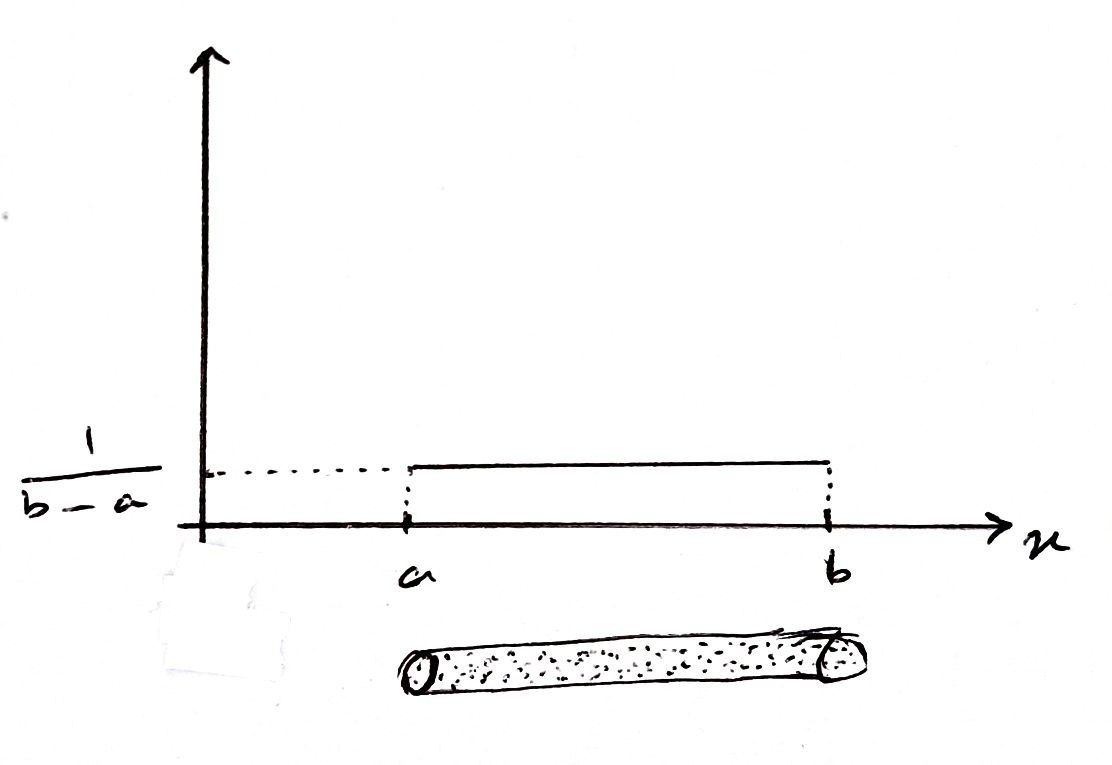
\epsfig{file=../img/uniformGraphWithRod.jpg,clip=true,width=8.8cm}
\end{center}
\caption{uniform distribution graph with unit-mass rod analogy}
\label{fig:uniform_graph}
%\HR
\end{figure}

\begin{exmp}
    A number is selected randomly between 3 and 7 (inclusive).
    \begin{enumerate}
        \item What is the probability that it equals 3.4?
        \item What is the probability that it lies between 4 and 6 (inclusive)?
    \end{enumerate}
\end{exmp}
\begin{solution}
    Let X be the selected number.
    Then \( \bm{X} \sim U(3, 7) \),
    and the PDF is \( f_{\bm{X}}(\bm{x}) = \frac{1}{7 - 3} = \frac{1}{4} \) where \( 3 \leq \bm{x} \leq 7 \).
    \begin{enumerate}
        \item \( P(\bm{X} = 3.4) = 0 \)
        \item \( P(4 \leq \bm{X} \leq 6) = (6 - 4) \times \frac{1}{4} = 0.5 \)
    \end{enumerate}
\end{solution}
